%-----------------------circuit 1--------------------------
\section{Single Phase Full Wave Uncontrolled Rectifier
  with R load}

\subsection{Circuit used for simulation}

% figure that is centered on the page
\begin{figure}[h]
    \centering
    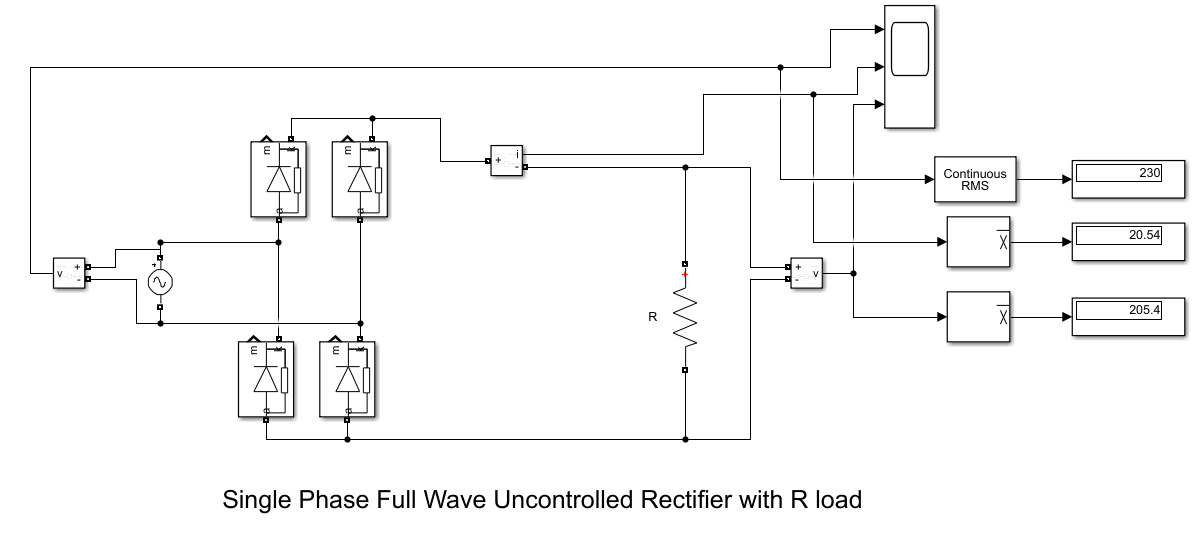
\includegraphics[width=0.7\textwidth]{images/experiment-2/circuit-diagram-simulation-01.png}
    \caption{Circuit used for simulation}
    \label{Fig_simulation_circuit_single-phase-full-wave-uncontrolled-rectifier-with-R-load}
\end{figure}

\subsection{Components Required}

\begin{table}[h]
    \renewcommand{\arraystretch}{1.3}
    \label{table_components_required_circuit_1}
    \centering
    \begin{tabular}{|c|c|c|c|}
        \hline
        Sr. No & Parameters                     & Ratings            & Quantity \\
        \hline
        \hline
        1      & AC Single Phase Voltage Source & 230V ($ V_{rms} $) & 1        \\
        \hline
        2      & Resistor                       & 10$ \Omega $       & 1        \\
        \hline
        3      & Diode                          & -                  & 1        \\
        \hline
        4      & Voltmeter                      & -                  & 2        \\
        \hline
        5      & Ammeter                        & -                  & 1        \\
        \hline
    \end{tabular}
    \caption{Components for Single Phase Full Wave Uncontrolled Rectifier with R load}

\end{table}




\subsection{Observations}

\begin{table}[h]
    \renewcommand{\arraystretch}{1.3}
    \label{table_observation_circuit_1}
    \centering
    \begin{tabular}{|c|c|c|}
        \hline
        Parameters                              & Theoretical Values & Simulation Values \\
        \hline
        \hline
        AC Input Voltage ($ V_{in,rms} $)       & 230V               & 230V              \\
        \hline
        Output Average Voltage ($ V_{o,avg} $)  & 207.07V            & 205.4V            \\
        \hline
        Output Average Current ($ I_{o,avg}  $) & 20.70A             & 20.54V            \\
        \hline
        DC Input Power ($ P_{DC}  $)            & 4218.916W          & 4173W             \\
        \hline
        Efficiency (\%)                         & 79.73              & 79.73             \\
        \hline
    \end{tabular}
    \caption{Observations for Single Phase Full Wave Uncontrolled Rectifier with R load}

\end{table}


The simulation results demonstrate that the theoretical values and the simulated values are almost identical. The circuit has a resistive load, which ensures that the output voltage and current are in phase. The full-wave rectification of the AC signal results in an output DC signal with twice the frequency of the input signal. This high-frequency DC signal can be advantageous in applications that require high-frequency power, such as in motor control circuits.
\pagebreak

\subsection{Resultant Waveforms}

% figure that is centered on the page
\begin{figure}[h]
    \centering
    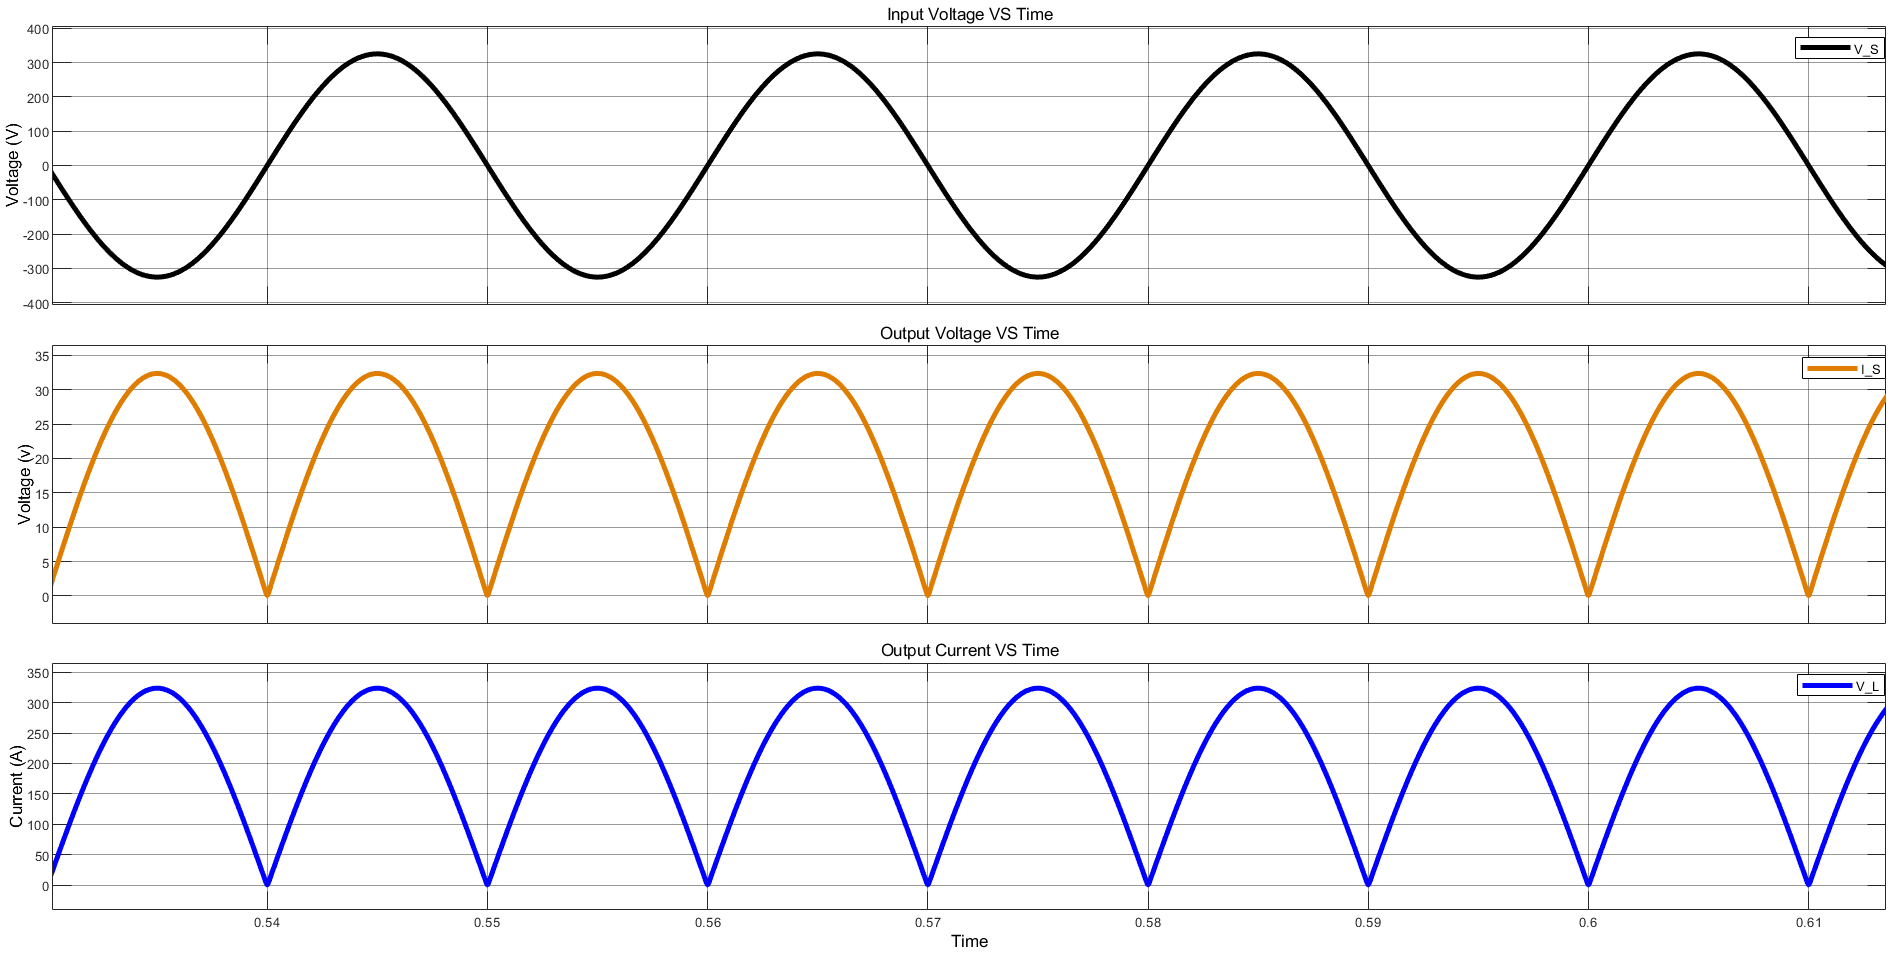
\includegraphics[width=1\textwidth]{images/experiment-2/circuit-scope-simulation-01.png}
    \caption{Scope Waveforms for Single Phase Full Wave Uncontrolled Rectifier with R load waveforms}
    \label{Fig_waveform_single-phase-full-wave-uncontrolled-rectifier-with-R-load}
\end{figure}

\pagebreak
